\documentclass[10pt]{article}
%-----------------------------------------------------------
\usepackage{geometry}
\usepackage{graphicx}   % need for figures
\usepackage{subfigure}
\usepackage[latin1]{inputenc}
\usepackage[parfill]{parskip} % To start a new paragraph with a blank line
%\usepackage[pdftex]{hyperref} %For url printing
\usepackage{setspace}
\usepackage{listings}
\onehalfspacing
\geometry{left=40mm,right=40mm,top=40mm,bottom=40mm}
\lstset{ 
	language=XML,               	% choose the language of the code
	basicstyle=\scriptsize,       % the size of the fonts that are used for the code
	numbers=left,                   % where to put the line-numbers
	numberstyle=\tiny,      		% the size of the fonts that are used for the line-numbers
	stepnumber=1,                   % the step between two line-numbers. If it's 1 each line will be numbered
	numbersep=5pt,                  % how far the line-numbers are from the code
	%backgroundcolor=\color{white},  % choose the background color. You must add \usepackage{color}
	%showspaces=false,               % show spaces adding particular underscores
	%showstringspaces=false,         % underline spaces within strings
	%showtabs=false,                 % show tabs within strings adding particular underscores
	frame=single,	                % adds a frame around the code
	tabsize=2,	                	% sets default tabsize to 2 spaces
	captionpos=b,                   % sets the caption-position to bottom
	%breaklines=true,                % sets automatic line breaking
	%breakatwhitespace=false,        % sets if automatic breaks should only happen at whitespace
	%escapeinside={\%*}{*)}          % if you want to add a comment within your code
}
%-----------------------------------------------------------
\title{TTSP - Tagus Time Synchronization Protocol}
\author{}
\date{}
%-----------------------------------------------------------
\begin{document}
\maketitle

\begin{center}
\begin{tabular}{ r l }
\textbf{Document} & Software Requirements Specification (SRS)\\
\textbf{Editor(s)} & Hugo Miguel Pinho Freire\\
\textbf{Contributor(s)}\\
\textbf{Institution(s)} & IST/TUL, GEMS/LEMe\\
\textbf{Version} & 1.2\\
\end{tabular}
\end{center}

\vspace{1cm}

\begin{abstract}
This document defines the software requirements for the development
of Tagus Time Synchronization Protocol (TTSP). TTSP is a time 
synchronization protocol for Wireless Sensor Networks (WSNs).
TTSP uses an adaptive approach to meet the time synchronization
requirements declared by the application.
The requirements specification of the time synchronization algorithm
used by TTSP and its prototype implementation will be detailed 
throughout this document.
The information collected in this document will be used as the 
basis for the next stages of the development process.
\end{abstract}

\clearpage
%-----------------------------------------------------------
\section*{Reviews}

\begin{center}
\begin{tabular}{ | c | l | l | p{6cm} | }
	\hline
	\textbf{Version} & \textbf{Date} & \textbf{Author} & \textbf{Comment}\\
	\hline
	1.0 & 13/02/10 & Hugo Miguel Pinho Freire & Initial draft\\
  1.1 & 27/02/10 & Hugo Miguel Pinho Freire & Updated references\\
  1.2 & 03/03/10 & Hugo Miguel Pinho Freire & Updated nonfunctional requirements\\  
	\hline
\end{tabular}
\end{center}

\clearpage
%-----------------------------------------------------------
\tableofcontents

\clearpage
%-----------------------------------------------------------
\addcontentsline{toc}{section}{List of Figures}
\listoffigures

\clearpage
%-----------------------------------------------------------
\addcontentsline{toc}{section}{List of Tables}
\listoftables

\clearpage
%-----------------------------------------------------------
\section*{List of Acronyms}
\addcontentsline{toc}{section}{List of Acronyms}

\begin{center}
\begin{tabular}{ r l }
AS & Assumption\\
CO & Constraint\\
FR & Functional Requirement\\
MAC & Medium Access Control \\
OE & Operating Environment \\
PR & Performance Requirement\\
TEP & TinyOS Enhancement Proposals \\
TSN & Tagus-SensorNet \\
TTSP & Tagus Time Synchronization Protocol \\
WSN & Wireless Sensor Network \\
\end{tabular}
\end{center}

\clearpage
%-----------------------------------------------------------
\section{Introduction \label{sec:introduction}}

\subsection{Purpose}
This document defines the software functional and nonfunctional
requirements for release version 1.0 of the Tagus Time 
Synchronization Protocol (TTSP). This document is intended to
be used by the author of TTSP (or other intended developers)
and will allow  it's implementation and the verification of
the correct functioning of the the system.

\subsection{Document Conventions}
MUST, SHALL and REQUIRED are used for requirements which have
been identified as critical and cannot be sidestepped.
SHOULD and RECOMMENDED are used for requirements that would
be desirable but may not be included, pending further 
evaluation. MAY and OPTIONAL are used for requirements that
are fully optional and that will only be implemented if judge
useful, interesting and not too demanding.

\subsection{Project Scope}
TTSP will permit WSN nodes to synchronize their local time
clocks (oscillator driven) with other WSN nodes, enabling a
global notion of time. TTSP delivers an adaptive time 
synchronization, in which sensor nodes try to achieve a time
precision error below a user specified value, typically the time
precision required by the application. This will allow for a 
better network and sensor node resource usage.

\subsection{References}

\begin{enumerate}
	\item Mar�ti M., Sallai J., TEP 133 - Packet-level time synchronization, http://www.tinyos.net/tinyos-2.x/doc/txt/tep133.txt
	\item Kus� B., Dutta P., Levis P., Mar�ti M., L�deczi �., Culler D., Elapsed time on arrival: a simple and versatile primitive for canonical time synchronization services, Int. J. Ad Hoc and Ubiquitous Computing, Vol. x, No. x, 200x
	\item Mar�ti M., Sallai J., TEP 132 - Packet timestamping, http://www.tinyos.net/tinyos-2.x/doc/txt/tep132.txt
\end{enumerate}

\clearpage
%-----------------------------------------------------------
\section{Overall Description \label{sec:description}}
\subsection{System Perspective}
TTSP is a time synchronization  protocol for WSNs, which will
be deployed into Tagus-SensorNet (TSN) sensor nodes in order 
deliver an adaptive time synchronization to it's applications 
and allow for a better network and sensor node resource usage
than the current available time synchronization protocols in TinyOS.
TTSP will be implemented in nesC as a component library of TinyOS in which
the applications shall wire to it in order to make use of TTSP
time synchronization features. 

\begin{figure}[!ht]
	\begin{center}
		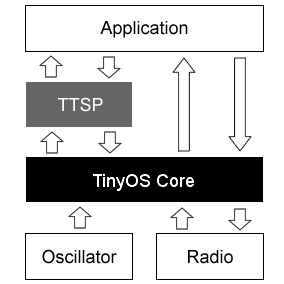
\includegraphics[width=6cm]{images/hfreire-ttsp-swhw.png}
	\end{center}
	\caption{TTSP interactions.}
	\label{swhw}
\end{figure}

TTSP interactions within a sensor node can be seen in Figure
\ref{swhw}. These interactions relate to the remaining software 
and hardware components that can be found in a typical sensor 
node running TinyOS.

\subsection{System Features}
Typical time synchronization protocols deliver a set of features
compromised in two distinct blocks: a pair-wise and network-wide 
time synchronization blocks. Pair-wise allows for 
one to synchronize a local pair of sensor nodes while network-wide
allows for the synchronization of the whole network,
specifically of sensor nodes that are multi-hop distance from each other.
Also, typical network-wide time synchronization features are built
on top of the pair-wise block, since it's solely
objective is to extend the synchronization between local neighbors
to the remaining multi-hop sensor nodes.

\begin{figure}[!ht]
	\begin{center}
		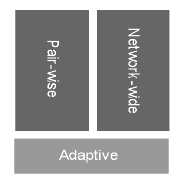
\includegraphics[width=6cm]{images/hfreire-ttsp-features.png}
	\end{center}
	\caption{TTSP features.}
	\label{features}
\end{figure}

That being said, as can be seen in Figure \ref{features}, TTSP
delivers a third block which is placed transversal to the
remaining blocks. This third block, adaptive
time synchronization, delivers features that make the current 
available features of pair-wise and network-wide to behave
in an adaptively fashion way.
The features of TTSP can be summarized in the following list:
\begin{itemize}
	\item Pair-wise time synchronization
	\item Network-wide time synchronization
	\item Adaptive time synchronization
\end{itemize}

\subsection{Operating Environment}
As previously said TTSP will be implemented in nesC as a component library
of TinyOS. Even though TinyOS has been evolving to create abstraction
layers between the application software and the hardware components,
it would be unwisely to assume that TTSP should work with every
sensor node that runs TinyOS. Mainly due to the specific need
to make special customizations in the MAC layer in order to
tweak TTSP performance. These customizations will be intrinsically 
associated with the respective radio interface. Thus, for now
TTSP will be implemented taking only into consideration the ChipCon CC2420 radio
that can be found on Crossbows MICAz sensor nodes. MICAz sensor nodes
have an Atmel micro-controller which will be programmed through an AVR GNU 
tool-chain.

\begin{table}[h!]
\begin{center}
\begin{tabular}{|c|c|c|}
\hline
Operating & \multicolumn{2}{|c|}{Description} \\
\cline{2-3}
Enviroment & Software & Version \\ \hline
OE-1 & TinyOS & 2.1.0 (possibly 2.1.1) \\ \hline
OE-2 & nesC & 1.3.0 \\ \hline
\end{tabular}
\caption{Software operating system and development language.}
\label{langos}
\end{center}
\end{table}

\begin{table}[h!]
\begin{center}
\begin{tabular}{|c|c|c|}
\hline
Operating & \multicolumn{2}{|c|}{Description} \\
\cline{2-3}
Enviroment & Software & Version \\ \hline
OE-3 & avr-gcc & 2.4 \\ \hline
OE-4 & avr-libc & 1.4.7 \\ \hline
OE-5 & avr-binutils & 2.17 \\ \hline
OE-6 & avr-insight & 6.3 \\ \hline
OE-7 & avrdude-tinyos & 5.6 \\ \hline
OE-8 & avarice & 2.4 \\ \hline
OE-9 & tinyos-tools & 1.30 \\ \hline
OE-10 & tinyos-deputy & 1.1 \\ \hline
\end{tabular}
\caption{Software cross-compiling tools.}
\label{swxtools}
\end{center}
\end{table}

Table \ref{langos} describes the operating system and
the development language that will be used to implement TTSP
while Table \ref{swxtools} describes the tools used for
cross-compiling TTSP to MICAz sensor nodes.

\begin{table}[h!]
\begin{center}
\begin{tabular}{|c|c|c|c|c|c|c|}
\hline
Operating & \multicolumn{5}{|c|}{Description} \\
\cline{2-6}
Enviroment & Sensor node & Processor & Flash size & RAM size & Radio throughput \\ \hline
OE-11 & MICAz & 8 MHz & 128 kB & 4 kB & 256 kbps  \\ \hline
\end{tabular}
\caption{Software cross-compilation tools.}
\label{micaz}
\end{center}
\end{table}

In Table \ref{micaz} it's possible to find a brief examination 
of Crossbows MICAz hardware capacity and denote its
scarce resources.

\subsection{Design and Implementation Constraints}
Typical design and implementation constraints of WSN protocols
apply to TTSP. Be it, the scarce memory resources and low processing power,
faulty and error prone communication links, faulty sensor nodes and
essentially energy limited batteries. 

\begin{table}[h!]
\begin{center}
\begin{tabular}{|c|l|}
\hline
Constraint & Description \\ \hline
CO-1 & Scarce memory resources \\ \hline
CO-2 & Low processing power \\ \hline
CO-3 & Faulty and error prone communication links \\ \hline
CO-4 & Energy limited batteries \\ \hline
\end{tabular}
\caption{Design and implementation constraints.}
\label{constraints}
\end{center}
\end{table}

The design and implementation constraints previously identified
are summarized in Table \ref{constraints}.
TTSP design should assume the existence of all these on a regular basis. 
Therefor the implementation should try to minimize the effect
that the following constraints have on TTSP execution:

\subsection{Assumptions and Dependencies}
The following assumptions listed here are to be taken into
consideration:

\begin{table}[h!]
\begin{center}
\begin{tabular}{|c|l|}
\hline
Assumption & Description \\ \hline
AS-1 & Every sensor node in the network has a unique ID \\ \hline
\end{tabular}
\caption{Assumptions and dependencies.}
\label{assumptdepend}
\end{center}
\end{table}

\clearpage
%-----------------------------------------------------------
\section{System Features}
\subsection{Pair-wise Synchronization}
\subsubsection{Description and Priority}
This feature is able to synchronize a pair of sensor nodes 
that are in the radio range of each other, thus synchronizing
through a single-hop communication. This feature is of HIGH
priority since it is the building block of a time synchronization
protocol.
The following items describe the main mechanisms
that are to be implemented by this feature:
\begin{itemize}
\item Synchronization through message exchange
\item MAC-layer timestamping
\item Synchronization in rounds, further known as synchronization points
\item Clock drif compensation
\end{itemize}

\subsubsection{Stimulus/Response Sequences}

\subsubsection{Functional Requirements}

\begin{table}[h!]
\begin{center}
\begin{tabular}{|c|p{10cm}|c|}
\hline
Requirement & Description & Priority \\ \hline
FR-1 & The system SHALL maintain an abstract notion of time, further known as global time & HIGH \\ \hline
FR-2 & The global time SHALL be expressed by the sum of local clock and an offset regarding another sensor node & HIGH \\ \hline
FR-3 & The offset SHALL be obtained by a sensor node after receiving the global time from a sender & HIGH \\ \hline
FR-4 & The global time of a sender SHALL be exchanged by messages transmitted over radio & HIGH \\ \hline
FR-5 & A sender MAY exchange messages with every receiving sensor node in its radio range & HIGH \\ \hline
FR-6 & Exchanged messages MUST carry the global time of the sender and its ID & HIGH \\ \hline
FR-7 & Exchanged messages SHOULD be time-stamped in the MAC layer at both the sender and in the receiver side & MEDIUM \\ \hline
FR-8 & Message exchange SHALL be done on a periodic basis, further known as synchronization points & HIGH \\ \hline
FR-9 & A pair <global time, local time>, further known as a reference point SHALL be stored for every synchronization point & HIGH \\ \hline
FR-10 & A sensor node SHALL start to discard the oldest reference points after a certain amount is reached & HIGH \\ \hline
FR-11 & The number of pairs to store before starting to discard is OPTIONAL & LOW \\ \hline
FR-12 & Compensation for the clock drift of the nodes SHALL be done in-between synchronization points & MEDIUM \\ \hline
FR-13 & Linear regression SHOULD be used for the compensation of the clock drift & HIGH \\ \hline
FR-14 & Linear regression SHALL make use of the stored reference points compensation of the clock drift & HIGH \\ \hline
FR-15 & A sensor nodes SHALL be synchronized when it has collected enough reference points to estimate its offset and drif of its own local clock & HIGH \\ \hline
\end{tabular}
\caption{Pair-wise synchronization functional requirements.}
\label{psyncfreq}
\end{center}
\end{table}

\subsection{Network-wide Synchronization}
\subsubsection{Description and Priority}
This feature is able to synchronize sensor nodes that are 
multi-hop distance from each other, thus away from each
other radio range. A controlled flooding mechanism and a
(re)election mechanism are used to provide a more
dynamic hierarchy structure, resilient to sensor node
failures or temporary link communication failures. This
feature is of HIGH priority since it allows for time
synchronization in multi-hop networks.
The following items describe the main mechanisms
that are to be implemented by this feature:
\begin{itemize}
\item Controlled flooding mechanism
\item Root (re)election mechanism
\end{itemize}

\subsubsection{Functional Requirements}

\begin{table}[h!]
\begin{center}
\begin{tabular}{|c|p{10cm}|c|}
\hline
Requirement & Description & Priority \\ \hline
FR-16 & Stored reference points MUST be only from a synchronization reference, further know as root & HIGH \\ \hline
FR-17 & Every sensor node SHALL take as root only one sensor node at a given point in time & HIGH \\ \hline
FR-18 & Root SHALL be dinamycally (re)elected, taking into account its ID & HIGH \\ \hline
FR-19 & Root (re)election SHALL be done regarding the lower ID of the sensor nodes & HIGH \\ \hline
FR-20 & Root (re)election SHALL be done by sensor nodes after a certain amount of time without receiving reference points from their root  & HIGH \\ \hline
FR-21 & The amount of time before considering the failure of the current root is OPTIONAL & MEDIUM \\ \hline
FR-21 & Only one root SHALL prevail after the election, although there may be more than one during the transition state & HIGH \\ \hline
FR-22 & Root sensor nodes after a synchronization point done by another root with a lesser ID SHALL drop its root status & HIGH \\ \hline
FR-23 & An ad-hoc structure SHALL be used to transfer the root global time to the remaining multi-hop distance sensor nodes & HIGH \\ \hline
FR-24 & A sensor node SHALL start to broadcast its global time after it has been synchronized & HIGH \\ \hline
\end{tabular}
\caption{Network-wide synchronization functional requirements.}
\label{nsyncfreq}
\end{center}
\end{table}

\subsection{Adaptive Synchronization}
\subsubsection{Description and Priority}
This feature is able to adapt the previously stated
features in order to reach below a specified precision
error. This precision error shall be specified either the
user at compile time or by the application itself during
runtime. This feature is of MEDIUM priority since it does
not affect the overall functionality of the time synchonization
protocol, but rather enhances its better resource usage.
Based on a number of reference points, every sensor node wants
to determine the largest interval between synchronization points such
that the synchronization error is smaller than the declared by the
application.

\subsubsection{Functional Requirements}
\begin{table}[h!]
\begin{center}
\begin{tabular}{|c|p{10cm}|c|}
\hline
Requirement & Description & Priority \\ \hline
FR-25 & Sensor nodes MUST be able to obtain the current periodicy of synchronization points. & HIGH \\ \hline
FR-26 & Sensor nodes SHALL calculate the optimal number of reference points that will provide the best drift estimation and prediction error. & HIGH \\ \hline
FR-27 & Sensor nodes SHALL gather the exact optimal number of reference points needed, and compute the drift estimation and prediction error. & HIGH \\ \hline
FR-28 & Using the prediction error the sensor node SHALL verify that it's under the synchronization error needed by the application & HIGH \\ \hline
FR-29 & If the predicted synchronization error is larger than the declared synchronization error, the sensor node SHALL broadcast a message stating a higher frequency & MEDIUM \\ \hline
FR-30 & If the predicted synchronization error is smaller than the declared synchronization error, the sensor node SHALL broadcast a message stating a lower frequency & MEDIUM \\ \hline
FR-31 & The root SHALL give priority to frequency increases than decreases & HIGH \\ \hline
FR-32 & The root SHALL use multiplicative increase and decrease strategies to adapt the frequency of the synchronization points & HIGH \\ \hline
\end{tabular}
\caption{Adaptive synchronization functional requirements.}
\label{asyncfreq}
\end{center}
\end{table}

\clearpage
%-----------------------------------------------------------
\section{External Interface Requirements}
\subsection{Hardware Interfaces}

\begin{table}[h!]
\begin{center}
\begin{tabular}{|c|p{10cm}|c|}
\hline
Requirement & Description & Priority \\ \hline
FR-20 & Red LED SHALL identify the transmission of a synchronization message & LOW \\ \hline
FR-21 & Green LED SHALL identify the reception of a synchronization message & LOW \\ \hline
FR-22 & Yellow LED SHALL identify the sensor node as being synchronized & LOW \\ \hline
\end{tabular}
\caption{Hardware interfaces requirements.}
\label{hwfreq}
\end{center}
\end{table}

%-----------------------------------------------------------
\section{Other Nonfunctional Requirements}
\subsection{Performance Requirements}

\begin{table}[h!]
\begin{center}
\begin{tabular}{|c|p{10cm}|c|}
\hline
Requirement & Description & Priority \\ \hline
PR-1 & The system MUST guarantee that a sensor node that boots is not unsynchronized for a extended period of time, no more than 60 seconds & LOW \\ \hline
\end{tabular}
\caption{Other nonfunctional requirements.}
\label{nfreq}
\end{center}
\end{table}

%-----------------------------------------------------------
\section{Other Requirements}

\begin{table}[h!]
\begin{center}
\begin{tabular}{|c|p{10cm}|c|}
\hline
Requirement & Description & Priority \\ \hline
OR-2 & The system SHALL be able to be aware of a network fresh boot and act upon it in order to speed the network-wide synchronization & LOW \\ \hline
OR-1 & The application MAY be able to modify the multiplicative factor in order to get a more fine grained control & LOW \\ \hline
\end{tabular}
\caption{Other requirements.}
\label{ofreq}
\end{center}
\end{table}

\clearpage
%-----------------------------------------------------------
\end{document}
